\documentclass{article}

\usepackage[utf8]{inputenc}

\usepackage{amsmath}
\usepackage{graphicx}
\usepackage{amssymb}
\usepackage{float}
\usepackage{caption}
\usepackage{subcaption}

\setlength{\parskip}{\baselineskip}%
\setlength{\parindent}{0pt}%

\begin{document}

\title{Materials Mini Project \\ \large{Packaging materials}}
\author{lwp26}
\date{October 2022}
\maketitle

\section{Abstract}
This is a report on a small project to investigate properties of foams and develop a method to select the best foam for a given application.
The report contains stress strain curves for a range of foams and a method to select the best foam for a given application based on theory discussed.
The report also contrains some microscopic imaging and example cases to demonstrate the selection method using the results obtained.


\section{Introduction}
Logistical networks are a fundamental part of our economy;
linking manufacturers, suppliers, wholesalers, retailers and consumers.
It is therefor important that these networks are efficient and reliable,
minimising cases of damage and loss of goods. Packaging is a key part of this,
as it protects goods from damage however it also adds weight and volume
which increases the costs of shipping.

\subsection{Packaging materials}
Packaging materials commonly consist of plastics, foams, cardboard and paper.
These materials are all relatively cheap and easy to produce, and all have relatively low densities.
Thin layers of plastic or corrugated cardboard provide a strong outer shell which
protects from peforation and crushing, while the foam or paper provides a cushion to absorb shock and vibration.
The materials are also relatively easy to recycle, and can be reused multiple times.

This report focuses on the use of foam as a packaging material.
\subsection{Aims}

\begin{itemize}
\item To investigate the properties of a range of foams and compare open and closed cell Foams
\item To develop a method for selecting packing foam materials for given applications
\end{itemize}

\section{Methodology and Theory}

The first scenario considered is a box containing an item of mass $m$ and area $A$ dropped at a height $h$.
% define fragility
The fragility of the item is defined as the maximum stress $\sigma_{max}$ it can withstand before breaking.
Fragile items have a low $\sigma_{max}$, while robust items have a high $\sigma_{max}$.

As the foam deforms on impact the foam moves along the stress-strain curve.
The energy absorbed by the foam per unit volume is given by the area under the stress-strain curve.
\begin{equation}
    \frac{mgh }{t A} = \int_{0}^{\varepsilon_{f}}\sigma d\varepsilon
\end{equation}
where $t$ is the thickness of the foam, $\varepsilon_f$ is the final strain.

Foams that can absorb most energy per unit while below $\sigma_{max}$ are the most suitable for fragile items.

This means that the minimum thickness of the foam is given by
\begin{equation}
    t = \frac{mgh}{A \int_0^{\varepsilon_{max}} \sigma d\varepsilon}
\end{equation}
where $\varepsilon_{max}$ is the strain at which the items stress is $\sigma_{max}$.

The goal is therefor to minimise the thickness of the foam while still absorbing enough energy to protect the item.
This means maximising the area under the stress-strain curve while still below $\sigma_{max}$.
This area encapsulated is the performance index of the foam.

Compression force displacement graphs of four foams were obtained experimentally using an Instron 68TM-30K machine.
The foam was compressed between a flat plate and a cylinder.
The force against displacement data was then used to calculate the stress-strain curves for each foam.



\section{Results}

\subsection{foams}

\begin{itemize}
    \item Ethafoam - Closed cell - $ 18.47 kg/m^3 $ - $0.1288$ MPa
    \item Polystyrene - Closed cell - $ 13.26 kg/m^3 $ - $0.2435$ MPa
    \item Polyurethane - Open cell - $ 26.39 kg/m^3 $ - $0.0235$ MPa
    \item White foam (Unknown material) - Closed cell - $20.3 kg/m^3 $ - $0.1729$ MPa
\end{itemize}
The elastic moduli of the foams were calculated from the largest linear region of the stress-strain curves.

\subsection{Foam characteristics}

\begin{figure}[H]
\centering
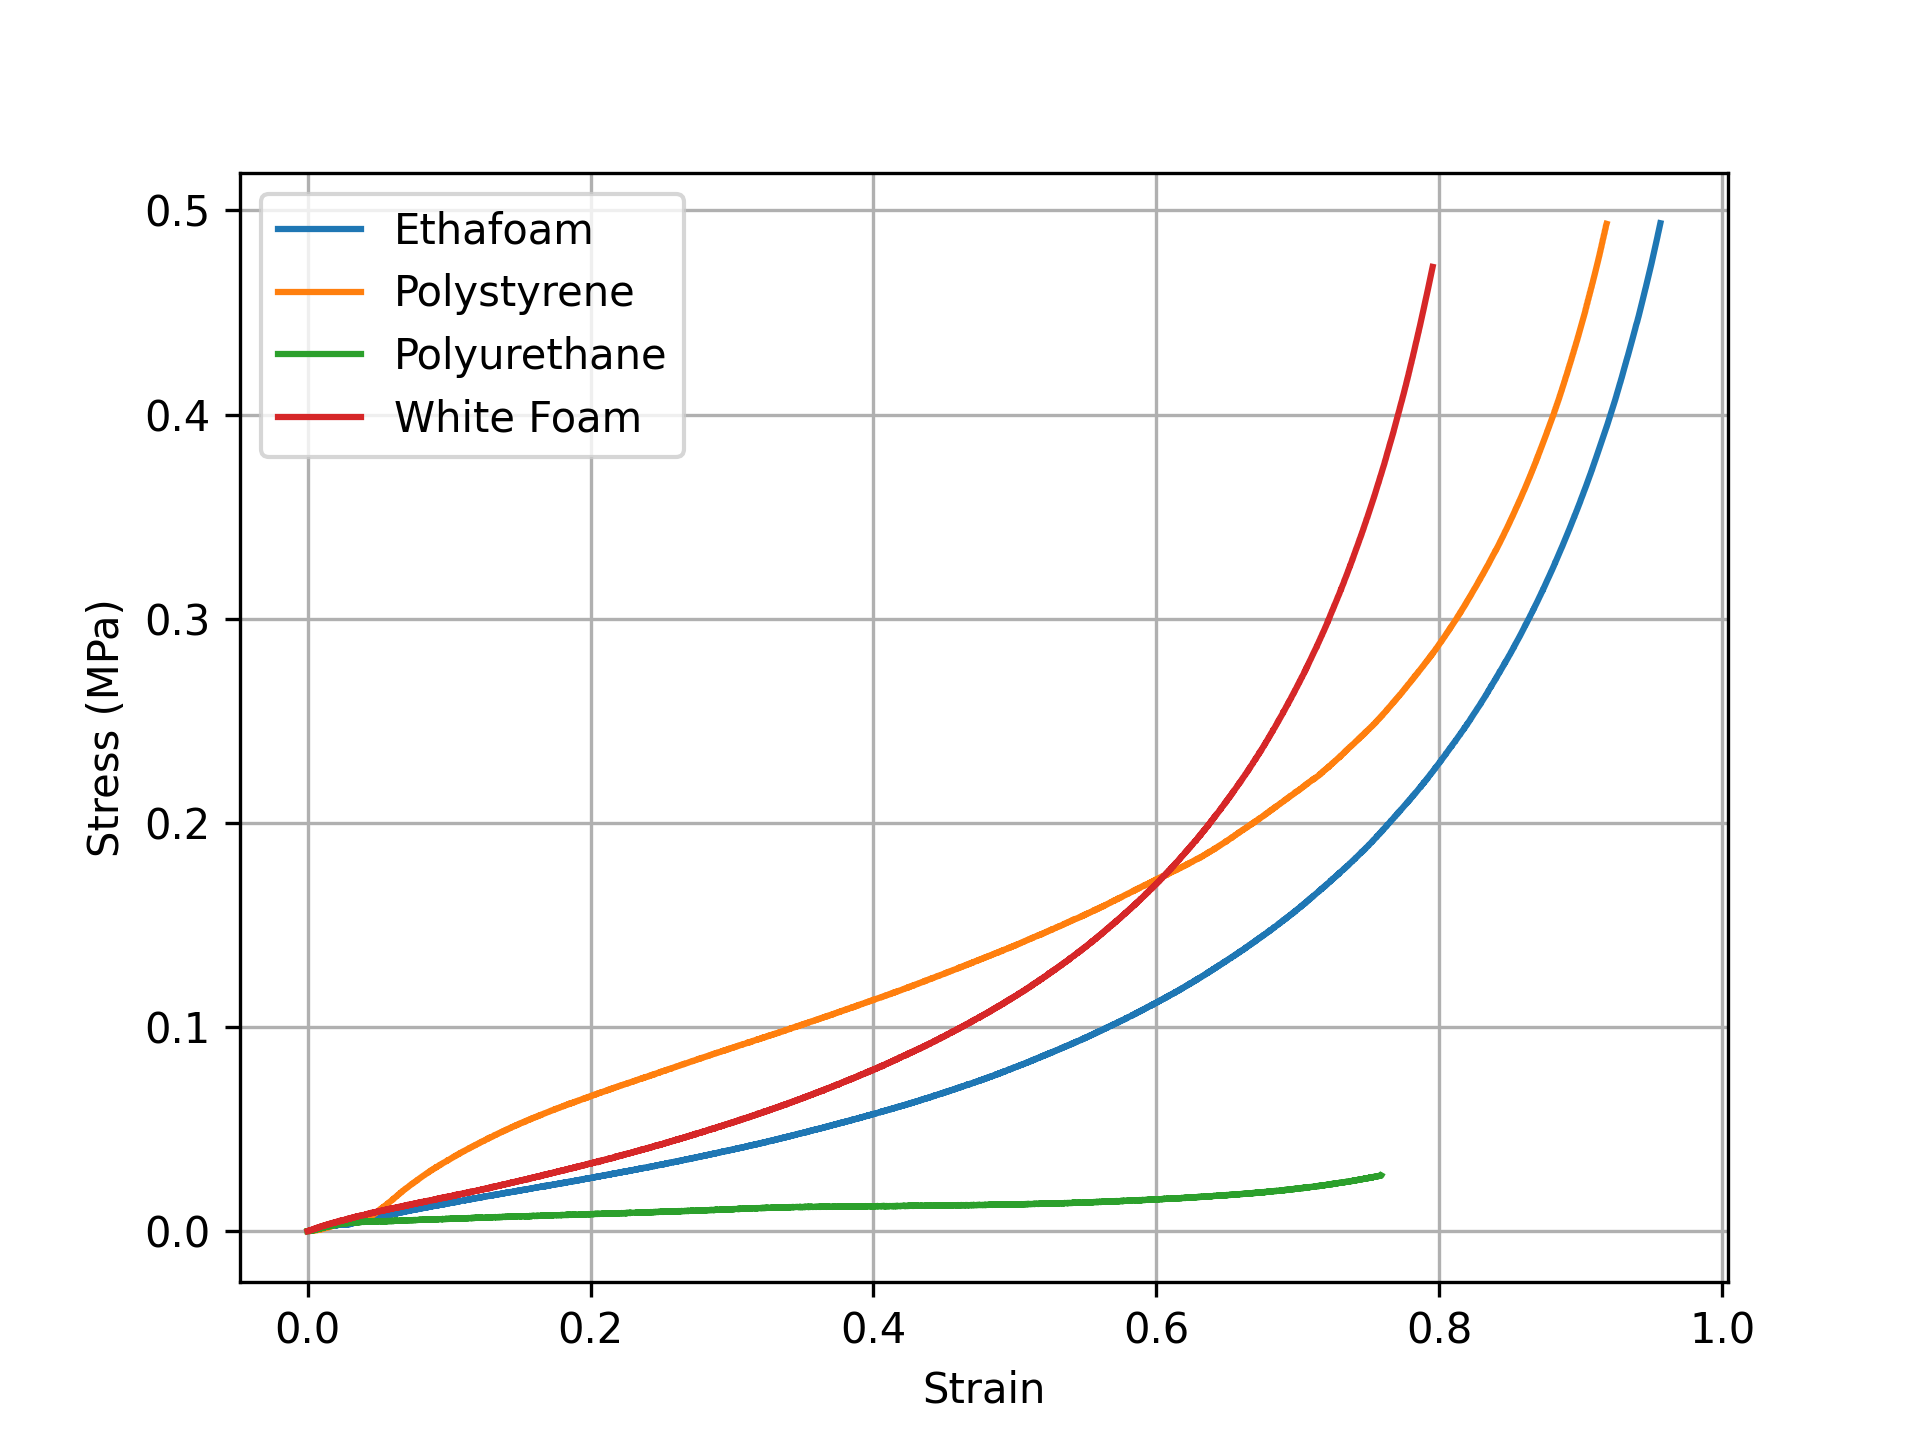
\includegraphics[width=1\textwidth]{stress_vs_strain.png}
\caption{\label{fig:stress_vs_strain} Graph of stress against strain for the foams}
\end{figure}

\begin{figure}[H]
\centering
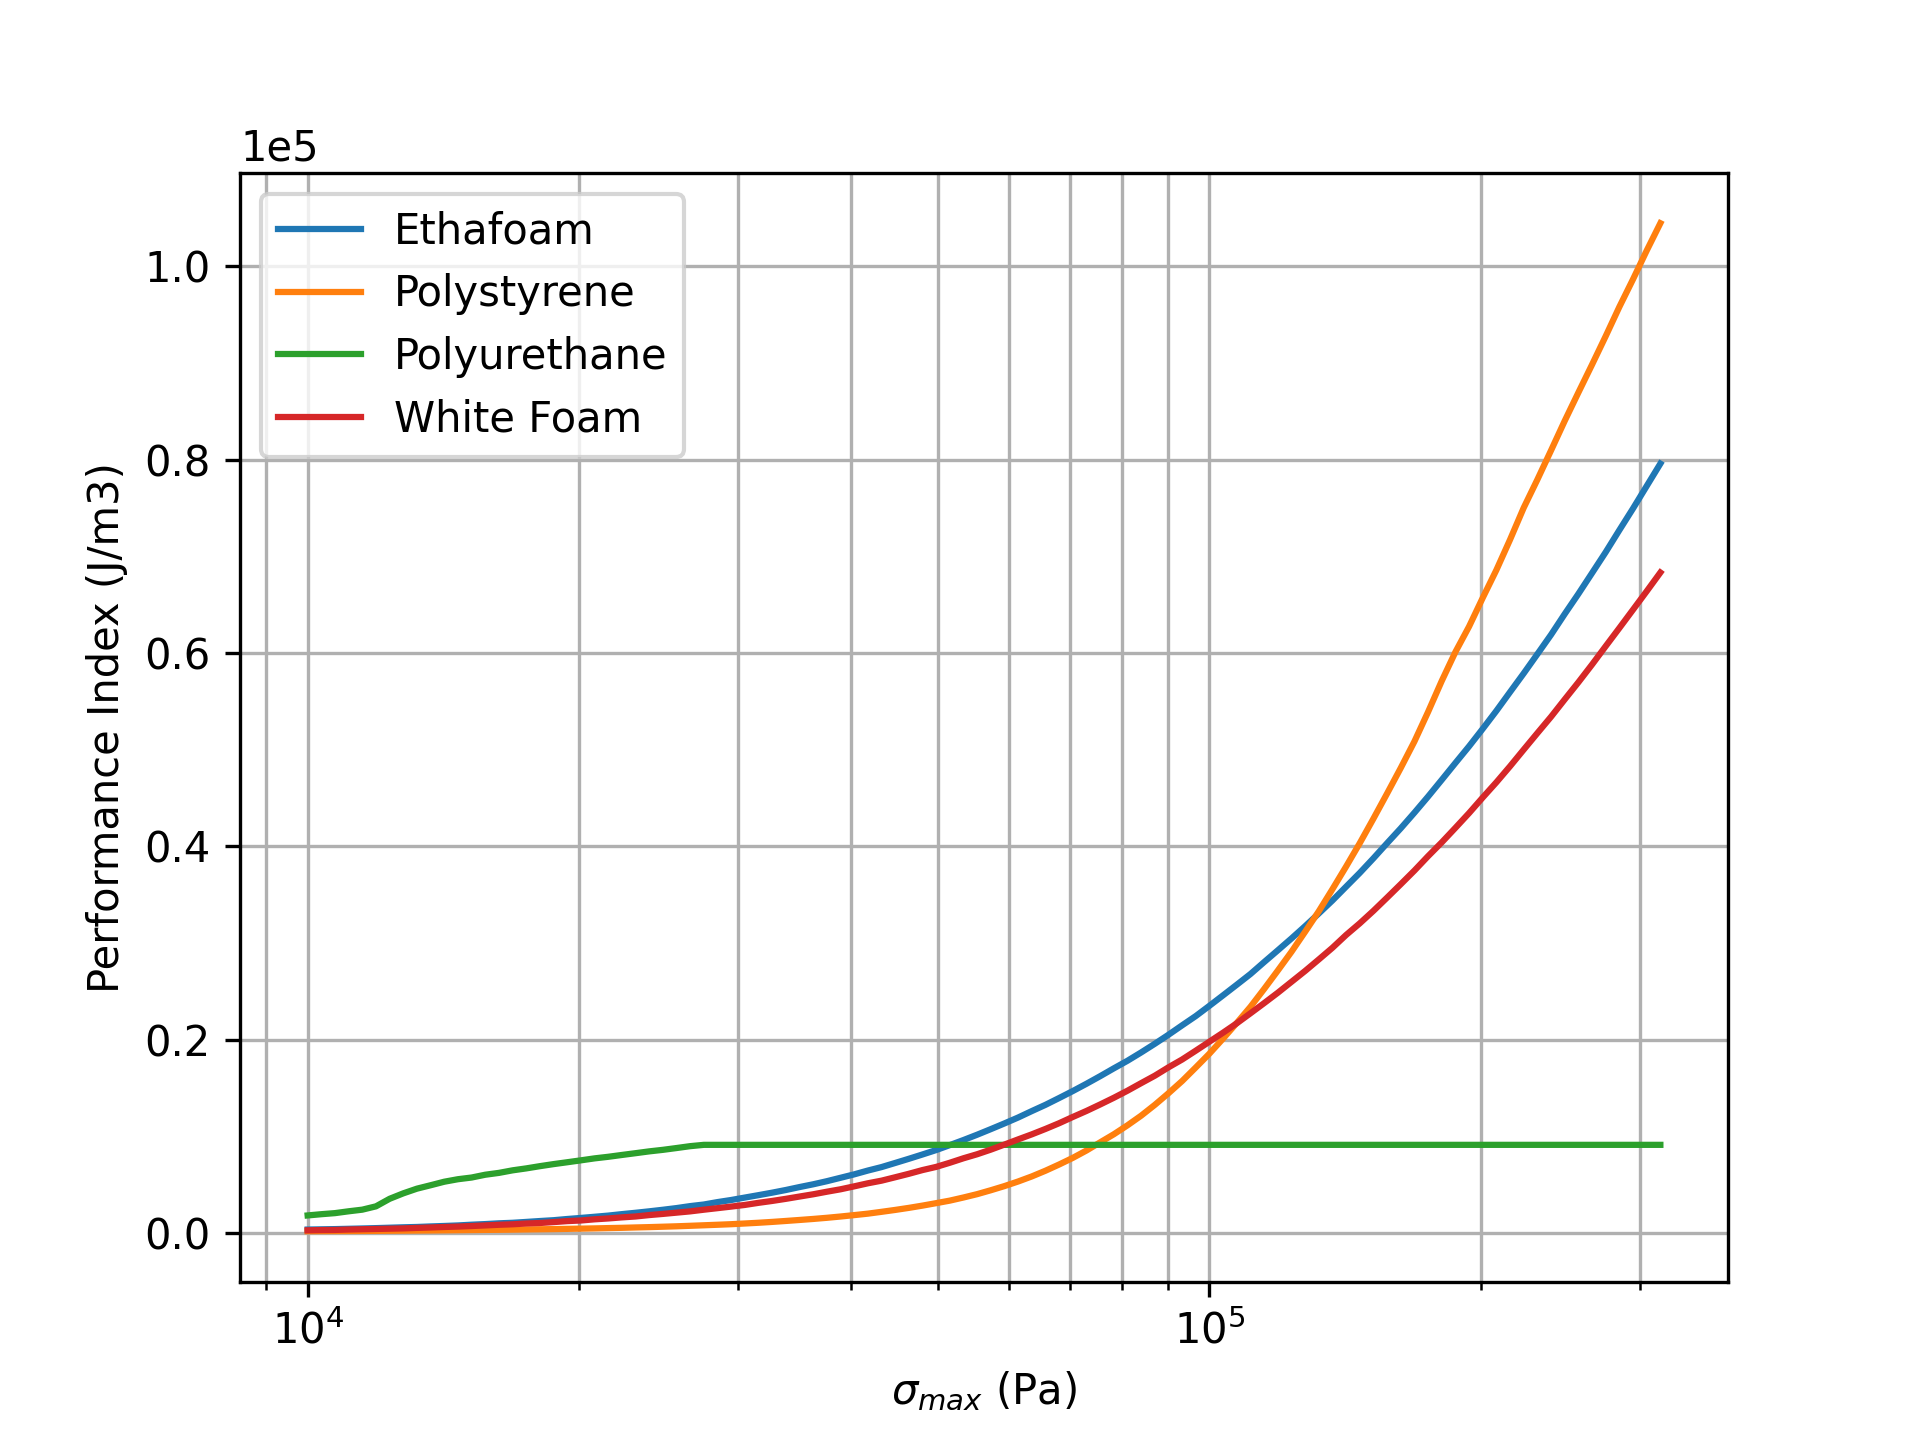
\includegraphics[width=1\textwidth]{vol_performance_vs_fragility.png}
\caption{\label{fig:vol_performance_vs_fragility} Graph of energy absorbed per unit volume against maximum allowable stress $\sigma_{max}$}
\end{figure}

\begin{figure}[H]
\centering
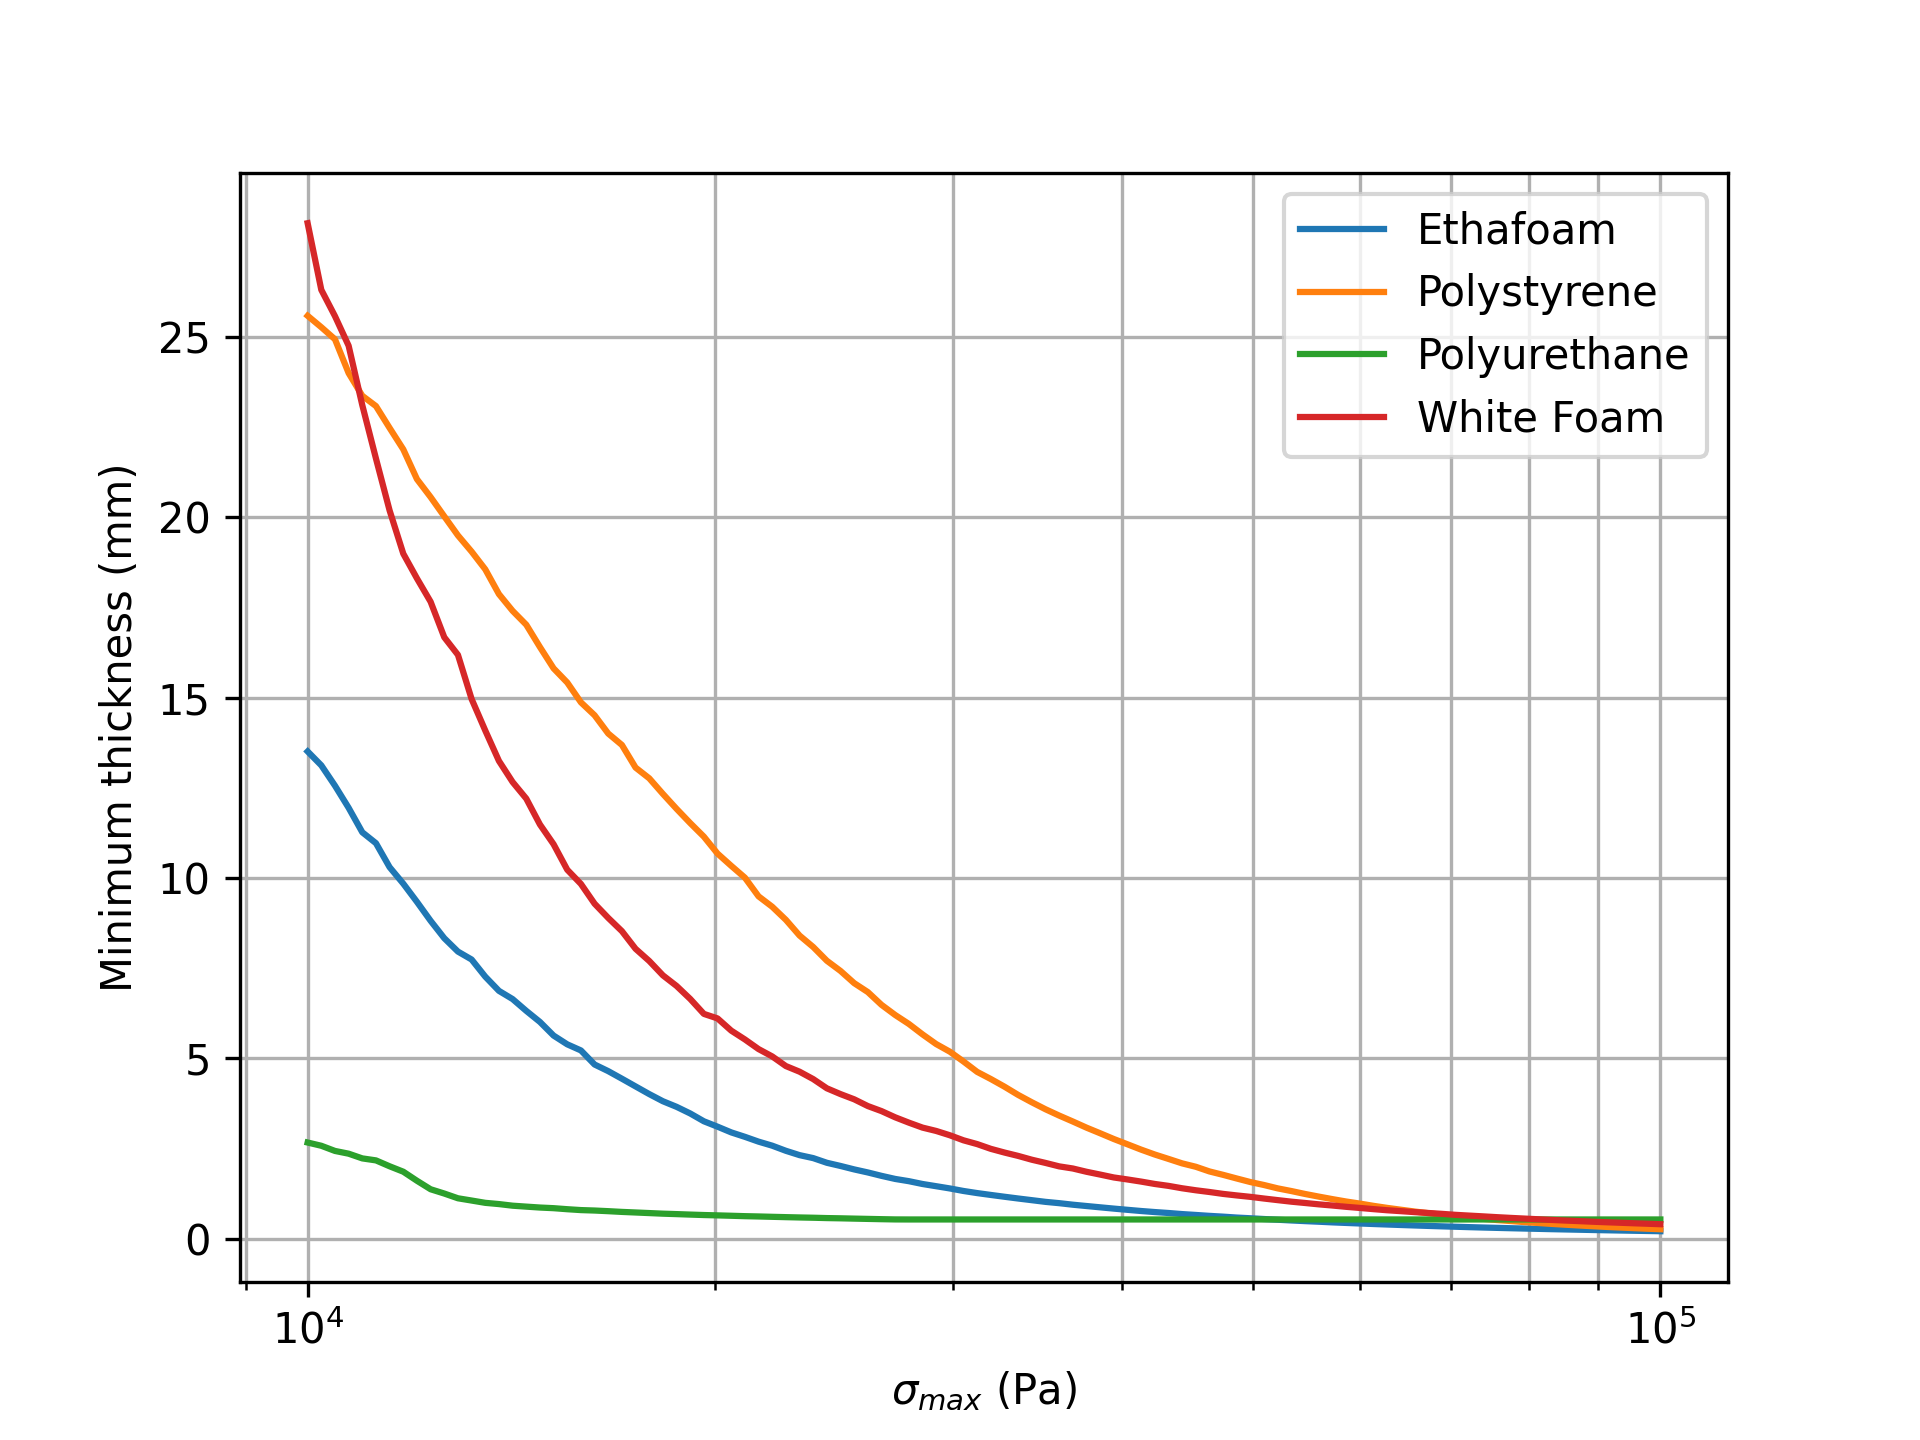
\includegraphics[width=1\textwidth]{thickness_vs_fragility.png}
\caption{\label{fig:thickness_vs_fragility} Graph of minimum thickness against maximum allowable stress $\sigma_{max}$}
\end{figure}

\subsection{Foam images}

\begin{figure}[H]
\centering
\includegraphics[width=0.8\textwidth]{17_polyurethane.png}
\caption{\label{fig:polyurethane} Polyurethane foam}
\end{figure}

\begin{figure}[H]
\centering
\includegraphics[width=0.8\textwidth]{17_white_foam.png}
\caption{\label{fig:white_foam} Dense white foam}
\end{figure}

\begin{figure}[H]
\centering
\includegraphics[width=0.8\textwidth]{17_ethafoam.png}
\caption{\label{fig:ethafoam} Ethafoam}
\end{figure}

\begin{figure}[H]
\centering
\subfloat[\centering compressed]{{\includegraphics[width=5cm]{17_polystyrene_compressed.png} }}%
\qquad
\subfloat[\centering uncompressed]{{\includegraphics[width=5cm]{17_polystyrene_uncompressed.png} }}%
\caption{\label{fig:polystyrene} Blown polystyrene before and after compression}
\end{figure}

\section{Discussion}

\subsection{Analysis of results}

The stress strain results show that all closed cell foams are stiffer than the open cell foam.
The open cell foam, polyurethane, also suprisingly has a higher density than the other foams.
This is due to air being able to escape from the foam during compression of the open foam.

From the performance index graph seen in figure \ref{fig:vol_performance_vs_fragility} it can be seen for fragile items $\sigma_{max} < 2\times 10^4 $ Pa the polyurethane is the best choice foam.
For robust items, $ \sigma_{max} < 9\times 10^4 $ Pa polystyrene is the most efficient choice of foam.
There is an area inbetween fragile and robust items at $ 9\times 10^4 < \sigma_{max} < 9\times 10^4 $ where ethafoam results in the best choice.

The difference of compressed and uncompressed polystyrene can be shown in figure \ref{fig:polystyrene}.
Unlike the other foams, polystyrene deforms permanantly at much lower strains.
Figure 7a shows the deformed blown polysyrene foam, including expansion lines as the 
foam has decompressed. Figure 7b shows the uncompressed foam, showing a more spherical shape.

\subsection{Limitations}

Many assumtions were made in calculations which can be improved upon in further testing.
One key assumption is that the elastic energy gained by the foam is equal to the energy lost by the item.
Another innacuracy arises from the foam not being constrained during compression.
In real world packages the foam is constrained by the box, and so the foam will not be able to expand as much as in the experiment.
This means in reality the foam will be stiffer than the experimentally measured values.
The youngs modulus of a constained material is given by

\begin{equation}
    E_{c} = \frac{E(1-\nu)}{1 - \nu - 2\nu^2}
\end{equation}

Foams have high poisson ratios, and so the constrained youngs modulus is much higher than the unconstrained value.
For $\nu = 0.25$ The constrained youngs modulus is $1.2$ times the unconstrained value.

Another assumption that was made was that the mass of the foam was negligible.
Fragile items require a large amount of foam to protect them.
This would increase the mass of the object and for light items this could be significant
enough to require more protective foam.

There were also limitations in the data that could be collected. The Instron machine that was used
could only perform quasistatic tests, meaning it was not possible to investigate impulse or harmonic foam responses.
This means it was not possible to investigate any damping properties of the foams for vibration testing.
There are also other scenarios of impulse loading that could be considered such as perforation.

\section{Example Cases}

\subsection{Mobile Phone}
A mobile phone can be modelled as a cuboid with dimensions $ 146.7 \times 71.5 \times 7.4 $ mm.
The phones mass is $ 0.162 $ kg and so $5g$ of acceleration corresponds to a force of about $8$N.
On the smallest face this gives a stress of $1.5\times 10^4$ Pa.
From figure \ref{fig:vol_performance_vs_fragility} we can see that the polyurethane foam is the best choice for this item.
The minimum thickness of the foam required can be found in figure \ref{fig:thickness_vs_fragility} to be about $ 1 $ mm.

\section{Conclusion}

The process for selecting an optimal foam for a given application is as follows:
\begin{itemize}
    \item Determine the maximum allowable force on a selected face
    \item Measure the area of the face
    \item Calculate the maximum allowable stress $\sigma_{max}$ of the item
    \item Find the foam with the highest energy absorbed per unit volume at $\sigma_{max}$ using figure \ref{fig:vol_performance_vs_fragility}
    \item Calculate the minimum thickness of the foam required to absorb the maximum force using equation (2)
    \item Repeat for all faces
\end{itemize}

This process developed can be used to select the most efficient foam for a given application and
be can used to determine the minimum thickness of the foam required to protect the item.
The limitations in testing and assumptions made in the analysis mean that the results should be treated with caution.
Further temporal based testing should be performed for confidence in a range of real world scenarios.
There are also many other factors that should be considered when selecting a foam such as cost, environmental impact, and recyclability.

\end{document}